\documentclass{article}

\usepackage{graphicx} % Required for inserting images
\usepackage[left=1in,right=1in,top=1in,bottom=1in]{geometry} \usepackage{amsmath}
\usepackage{amsthm} %proof environment
\usepackage{amsthm} %proof environment
\usepackage{amssymb}
\usepackage{amsfonts}
\usepackage{enumitem} %nice lists
\usepackage{verbatim} %useful for something 
\usepackage{xcolor}
\usepackage{setspace}
\usepackage{titlesec}
\usepackage{blindtext} % I have no idea what this is 
\usepackage{caption}  % need this for unnumbered captions/figures
\usepackage{natbib}
\usepackage{appendix}
\usepackage{tikz}
\usepackage{hyperref}


\hypersetup{
    colorlinks=true,
    linkcolor=blue,
    filecolor=magenta,      
    urlcolor=blue,
    pdftitle={Overleaf Example},
    pdfpagemode=FullScreen,
    }

\titleformat{\section}{\bfseries\Large}{Problem \thesection:}{5pt}{}

\begin{document}

\title{AM 216 - Stochastic Differential Equations: Assignment 3}
\author{Dante Buhl}


\newcommand{\wrms}{w_{\text{rms}}}
\newcommand{\bs}[1]{\boldsymbol{#1}}
\newcommand{\tb}[1]{\textbf{#1}}
\newcommand{\bmp}[1]{\begin{minipage}{#1\textwidth}}
\newcommand{\emp}{\end{minipage}}
\newcommand{\R}{\mathbb{R}}
\newcommand{\C}{\mathbb{C}}
\newcommand{\N}{\mathcal{N}}
\newcommand{\Var}{\text{Var}}
\newcommand{\Cov}{\text{Cov}}
\newcommand{\Bino}{\text{Bino}}
\newcommand{\Norm}{\mathcal{N}}
\newcommand{\erf}{\text{erf}}
%\newcommand{\K}{\bs{\mathrm{K}}}
\newcommand{\m}{\bs{\mu}_*}
\newcommand{\s}{\bs{\Sigma}_*}
\newcommand{\dt}{\Delta t}
\newcommand{\dx}{\Delta x}
\newcommand{\tr}[1]{\text{Tr}(#1)}
\newcommand{\Tr}[1]{\text{Tr}(#1)}
\newcommand{\Div}{\nabla \cdot}
\renewcommand{\div}{\nabla \cdot}
\newcommand{\Curl}{\nabla \times}
\newcommand{\Grad}{\nabla}
\newcommand{\grad}{\nabla}
\newcommand{\grads}{\nabla_s}
\newcommand{\gradf}{\nabla_f}
\newcommand{\xs}{x_s}
\newcommand{\x}{\bs{x}}
\newcommand{\xf}{x_f}
\newcommand{\ts}{t_s}
\newcommand{\tf}{t_f}
\newcommand{\pt}{\partial t}
\newcommand{\pz}{\partial z}
\newcommand{\uvec}{\bs{u}}
\newcommand{\bvec}{\bs{B}}
\newcommand{\nvec}{\hat{\bs{n}}}
\newcommand{\tu}{\tilde{\uvec}}
\newcommand{\B}{\bs{B}}
\newcommand{\A}{\bs{A}}
\newcommand{\jvec}{\bs{j}}
\newcommand{\F}{\bs{F}}
\newcommand{\T}{\tilde{T}}
\newcommand{\ez}{\bs{e}_z}
\newcommand{\ex}{\bs{e}_x}
\newcommand{\ey}{\bs{e}_y}
\newcommand{\eo}{\bs{e}_{\bs{\Omega}}}
\newcommand{\ppt}[1]{\frac{\partial #1}{\partial t}}
\newcommand{\pp}[2]{\frac{\partial #1}{\partial #2}}
\newcommand{\pptwo}[2]{\frac{\partial^2 #1}{\partial #2^2}}
\newcommand{\ddtwo}[2]{\frac{d^2 #1}{d #2^2}}
\newcommand{\DDt}[1]{\frac{D #1}{D t}}
\newcommand{\ppts}[1]{\frac{\partial #1}{\partial t_s}}
\newcommand{\pptf}[1]{\frac{\partial #1}{\partial t_f}}
\newcommand{\ppz}[1]{\frac{\partial #1}{\partial z}}
\newcommand{\ddz}[1]{\frac{d #1}{d z}}
\newcommand{\ppzetas}[1]{\frac{\partial^2 #1}{\partial \zeta^2}}
\newcommand{\ppzs}[1]{\frac{\partial #1}{\partial z_s}}
\newcommand{\ppzf}[1]{\frac{\partial #1}{\partial z_f}}
\newcommand{\ppx}[1]{\frac{\partial #1}{\partial x}}
\newcommand{\ddx}[1]{\frac{d #1}{d x}}
\newcommand{\ppxi}[1]{\frac{\partial #1}{\partial x_i}}
\newcommand{\ppxj}[1]{\frac{\partial #1}{\partial x_j}}
\newcommand{\ppy}[1]{\frac{\partial #1}{\partial y}}
\newcommand{\ppzeta}[1]{\frac{\partial #1}{\partial \zeta}}
\renewcommand{\k}{\bs{k}}
\newcommand{\real}[1]{\text{Re}\left[#1\right]}


\maketitle 
% This line removes the automatic indentation on new paragraphs
\setlength{\parindent}{0pt}

\section{Fair Gambler's Ruin}
    \begin{proof}
        \begin{align*}
            u(x,t) &= Pr(X(\tau) > 0, \tau \in [0,t] \& X(t) > c_0 | X(0) =
            x)\\
            &= E(Pr(A | X(dt) = x + dW) + d(dt)\\
            &= E(u(x+dW, t-dt))\\
            &= E\left[u(x,t) + u_x dW - u_t dt + u_{xx}dW^2/2 +
            o(dt^{3/2})\right]\\
            &= u(x,t) - u_tdt + u_{xx}dt/2\\
            u_t &= \frac{1}{2}u_xx
            \\
            u(0,t) = 0, &\quad u(x,0) = \begin{cases}1 & x > c_0\\0 &
            0<x<c_0\end{cases}
        \end{align*}
    \end{proof}

\section{Solving the IBVP}
    \begin{enumerate}[label=\roman*)]
        \item We use the odd extension, 
        \begin{align*}
            u_t &= \frac{1}{2}u_xx
            \\
            u(0,t) = 0, &\quad u(x,0) = \begin{cases}1 & x > c_0\\0 &
            -c_0<x<c_0\\ -1 & x < -c_0\end{cases}
        \end{align*}
        \item 
        \begin{align*}
            u(x,t) &= \frac{1}{\sqrt{2\pi t}} \int_{-\infty}{\infty}
            e^{-\xi^2/2t} f(x-\xi)d\xi\\
            &= \frac{1}{\sqrt{2\pi t}} \int_{-\infty}{x-c_0}
            e^{-\xi^2/2t}d\xi - \int_{x + c_0}{\infty}
            e^{-\xi^2/2t}d\xi
        \end{align*}
        \item 
            By a goemetric argument we can state that $d = x+c_0$ and $b =
            |x-c_0|$, $a = d-b$ (note that we are guaraneed $d > 0$). 
            \begin{align*}
                u(x,t) &= \frac{1}{\sqrt{2\pi t}} \int_0^a e^{\xi^2/2t}d\xi 
                \\
                &= \frac{1}{2}\erf\left(\frac{a}{\sqrt{2t}}\right)
                \\
                &= \frac{1}{2}\erf\left(\frac{x+c_0 - |x-c_0|}{\sqrt{2t}}\right)
            \end{align*}
    \end{enumerate}

\section{Solve the BVP}
    \begin{enumerate}[label=\roman*)]
        \item We have, 
        \begin{align*}
            \frac{d}{dx}\left(T_x - 2mT\right) &= -2
            \\
            \left(T_x - 2mT\right) &= -2x + c
            \\
            e^{-2mx}\left(T_x - 2mT\right) &= (-2x + c)e^{-2mx}
            \\
            e^{-2mx}T &= \int (-2x+c)e^{-2mx}dx
            \\
            T(x) &= e^{2mx}\int (-2x+c)e^{-2mx}dx
            \\
            &= e^{2mx}\left(ce^{-2mx} + \frac{x}{m}e^{-2mx} +
            \frac{1}{2m^2}e^{-2mx} + c_2\right)
            \\
            &= c + \frac{x}{m} + \frac{1}{2m^2} + c_2e^{2mx}
            \\
            &= \frac{x}{m} - \frac{C}{m}\left(\frac{e^{2mx} - 1}{e^{2mC} -
            2}\right), \quad (\text{applying BC})
        \end{align*}
        where solving for the BC looks like
        \begin{align*}
            T(0) &= c_1 + 0 + \frac{1}{2m^2} + c_2 = 0\\
            T(C) &= c_1 + \frac{C}{m} + \frac{1}{2m^2} + c_2e^{2mC} = 0\\
            c_1 &= -c_2 - \frac{1}{2m^2}
            \\
            0 &= \frac{C}{m} + c_2\left(e^{2mC} - 1\right)
            \\
            c_2 &= -\frac{C}{m}\left(e^{2mC} - 1\right)^{-1}
            \\
            T(x) &= \frac{x}{m} - \frac{C}{m}\frac{e^{2mx} - 1}{e^{2mC} - 1}
        \end{align*}
    \end{enumerate}

\section{Confirming Ito's Lemma}
    \begin{enumerate}[label=\roman*)]
        \item 
        \begin{align*}
            E(X_j^4) &=\frac{1}{\sqrt{2\pi}} \int_{-\infty}^{\infty} x^4e^{-x^2/2}dx
            \\
            &= \sqrt{\frac{2}{\pi}} \int_{0}^{\infty}
            x^3\left(xe^{-x^2/2}\right)dx\\
            &=  \sqrt{\frac{2}{\pi}} 3\int_{0}^{\infty}
            x\left(xe^{-x^2/2}\right)dx\\
            &= \sqrt{\frac{2}{\pi}} 3\int_{0}^{\infty}
            e^{-x^2/2}dx\\
            &= 3
            \\
            E(dW_j^4) &= E((\sqrt{dt})^4X_j) = 3dt^2
        \end{align*}
        \item Since each $dW_j$ is iid we have,
        \begin{align*}
            E(Q_n) &= \sum_{j=0}^{n-1} E(2t_jdW_j^2)\\
            &= \sum_{j=0}^{n-1} 2t_jE(dW_j^2) 
            \\
            &= \sum_{j=0}^{n-1} 2t_jdt
            \\
            \Var(Q_n) &=\sum_{j=0}^{n-1} \Var(2t_jdW_j^2) \\
            &=   \sum_{j=0}^{n-1} 4t_j^2\Var(dW_j^2)
            \\
            &=   \sum_{j=0}^{n-1} 4t_j^2dt^2\Var(X_j^2)
            \\
            &=   \sum_{j=0}^{n-1} 8t_j^2dt^2
            \\
            \lim_{n\to\infty}\sum_{j=0}^{n-1} 2t_jdt &=
            \lim_{n\to\infty}\frac{2t_f^2}{n^2}\sum_{j=0}^{n-1} j
            \\
            &= \lim_{n\to\infty}\frac{2t_f^2}{n^2}(n-1)(n-2)/2
            \\
            &= t_f^2 = \int_0^{t_f} 2tdt
            \\
            \lim_{n\to\infty}\Var(Q_n) &=  \frac{8t_f^4}{n^4}\sum_{j=0}^{n-1} j^2 
            \\
            &= \frac{8t_f^4}{n^4}O(n^3) = 0 
        \end{align*}
    \end{enumerate}

\section{Showing brownian motion is iid}
    \begin{enumerate}[label=\roman*)]
        \item We begin by writing $X1 = W_3 - W_2$, $X2 = W_2 - W_1$ and $Y =
        W1$. 
        We attempt to show that $P(X1|X2,Y) = P(X_1)$. 
        \begin{align*}
            P(X1|X2,Y) &= \frac{P(X1,X2 \& Y)}{P(X2 \& Y}
            \\
            &= \frac{P(X1)P(X2)P(Y)}{P(X2)P(Y)} = P(X1)
        \end{align*}
        where this simplification requires that we know that $X1$ and $X2$ are
        iid by the definition of brownian motion and that neither $X1$ and $X2$
        depend on $Y$ (since they are distributed as $N(0,dt)$). 
        This shows that $X1$ is independent of $X2$ and $Y$ and more
        specifically, 
        $W_3 \sim W_2 + \sqrt{dt}N(0,1) = N(W_2,dt)$
        Therefore we can make the statement, 
        \[(W(t_3)|W(t_2) = w_2, W(t_1) = w_1) \sim (W(t_3)|W(t_2) = w_2)\]
        \item The same argument holds for 
        \[(W(t_2)|W(t_3) = w_3, W(t_4) = w_4) \sim (W(t_2)|W(t_3) = w_3)\]
        except here we define $X1 = W_2 - W_3$, $X2 = W_3 - W_4$, and $Y = W4$.
        The same exact argument holds and there is no sign change because the
        brownian increment is symmetrically distributed about zero (i.e. $dW_{32}
        \sim dW_{23}$)
    \end{enumerate}

\section{Stationary Process}
    \begin{align*}
        R(\tau) &= E(Z(s+\tau)Z(s))
        \\
        &= \frac{1}{\Delta t^2}E\left[
        (W(s + \tau + \Delta t)-W(s + \tau))(W(s + \Delta t)-W(s))\right]
        \\
        &= \frac{1}{\Delta t^2}E\left[
        (a - b)(b - c)\right],\quad a = W(s + \tau + \Delta t)-W(s + \Delta t)
        \\
        b = W(s + \Delta t) - W(s + \tau) & \quad c = W(s + \tau) - W(s)
        \\
        &= \frac{1}{\Delta t^2}E\left[ab + ac + bb + bc\right]
        \\
        &= \frac{1}{\Delta t^2}E\left[bb\right] = \frac{\Delta t - \tau}{\Delta
        t^2}
    \end{align*}
    This is, of course, for the case where $\Delta t > \tau$ and so the
    differences $dW$ are not independent, i.e. there is some overlap in the two
    differences in time. In the case where $\tau > \Delta t$ there is no overlap
    and the two differences are independent and identically distributied as
    $N(0,dt)$. That is, $R(\tau) = 0$ when $\tau > \Delta t$. 

\section{Numerical Itos Lemma}
    \begin{enumerate}[label=\roman*)]
        \item See Figure \ref{fig:p7pb}
        \item See Figure \ref{fig:p7pb}
        \item See Figure \ref{fig:p7pc}
    \end{enumerate}
\begin{figure}[th]
    \centering
    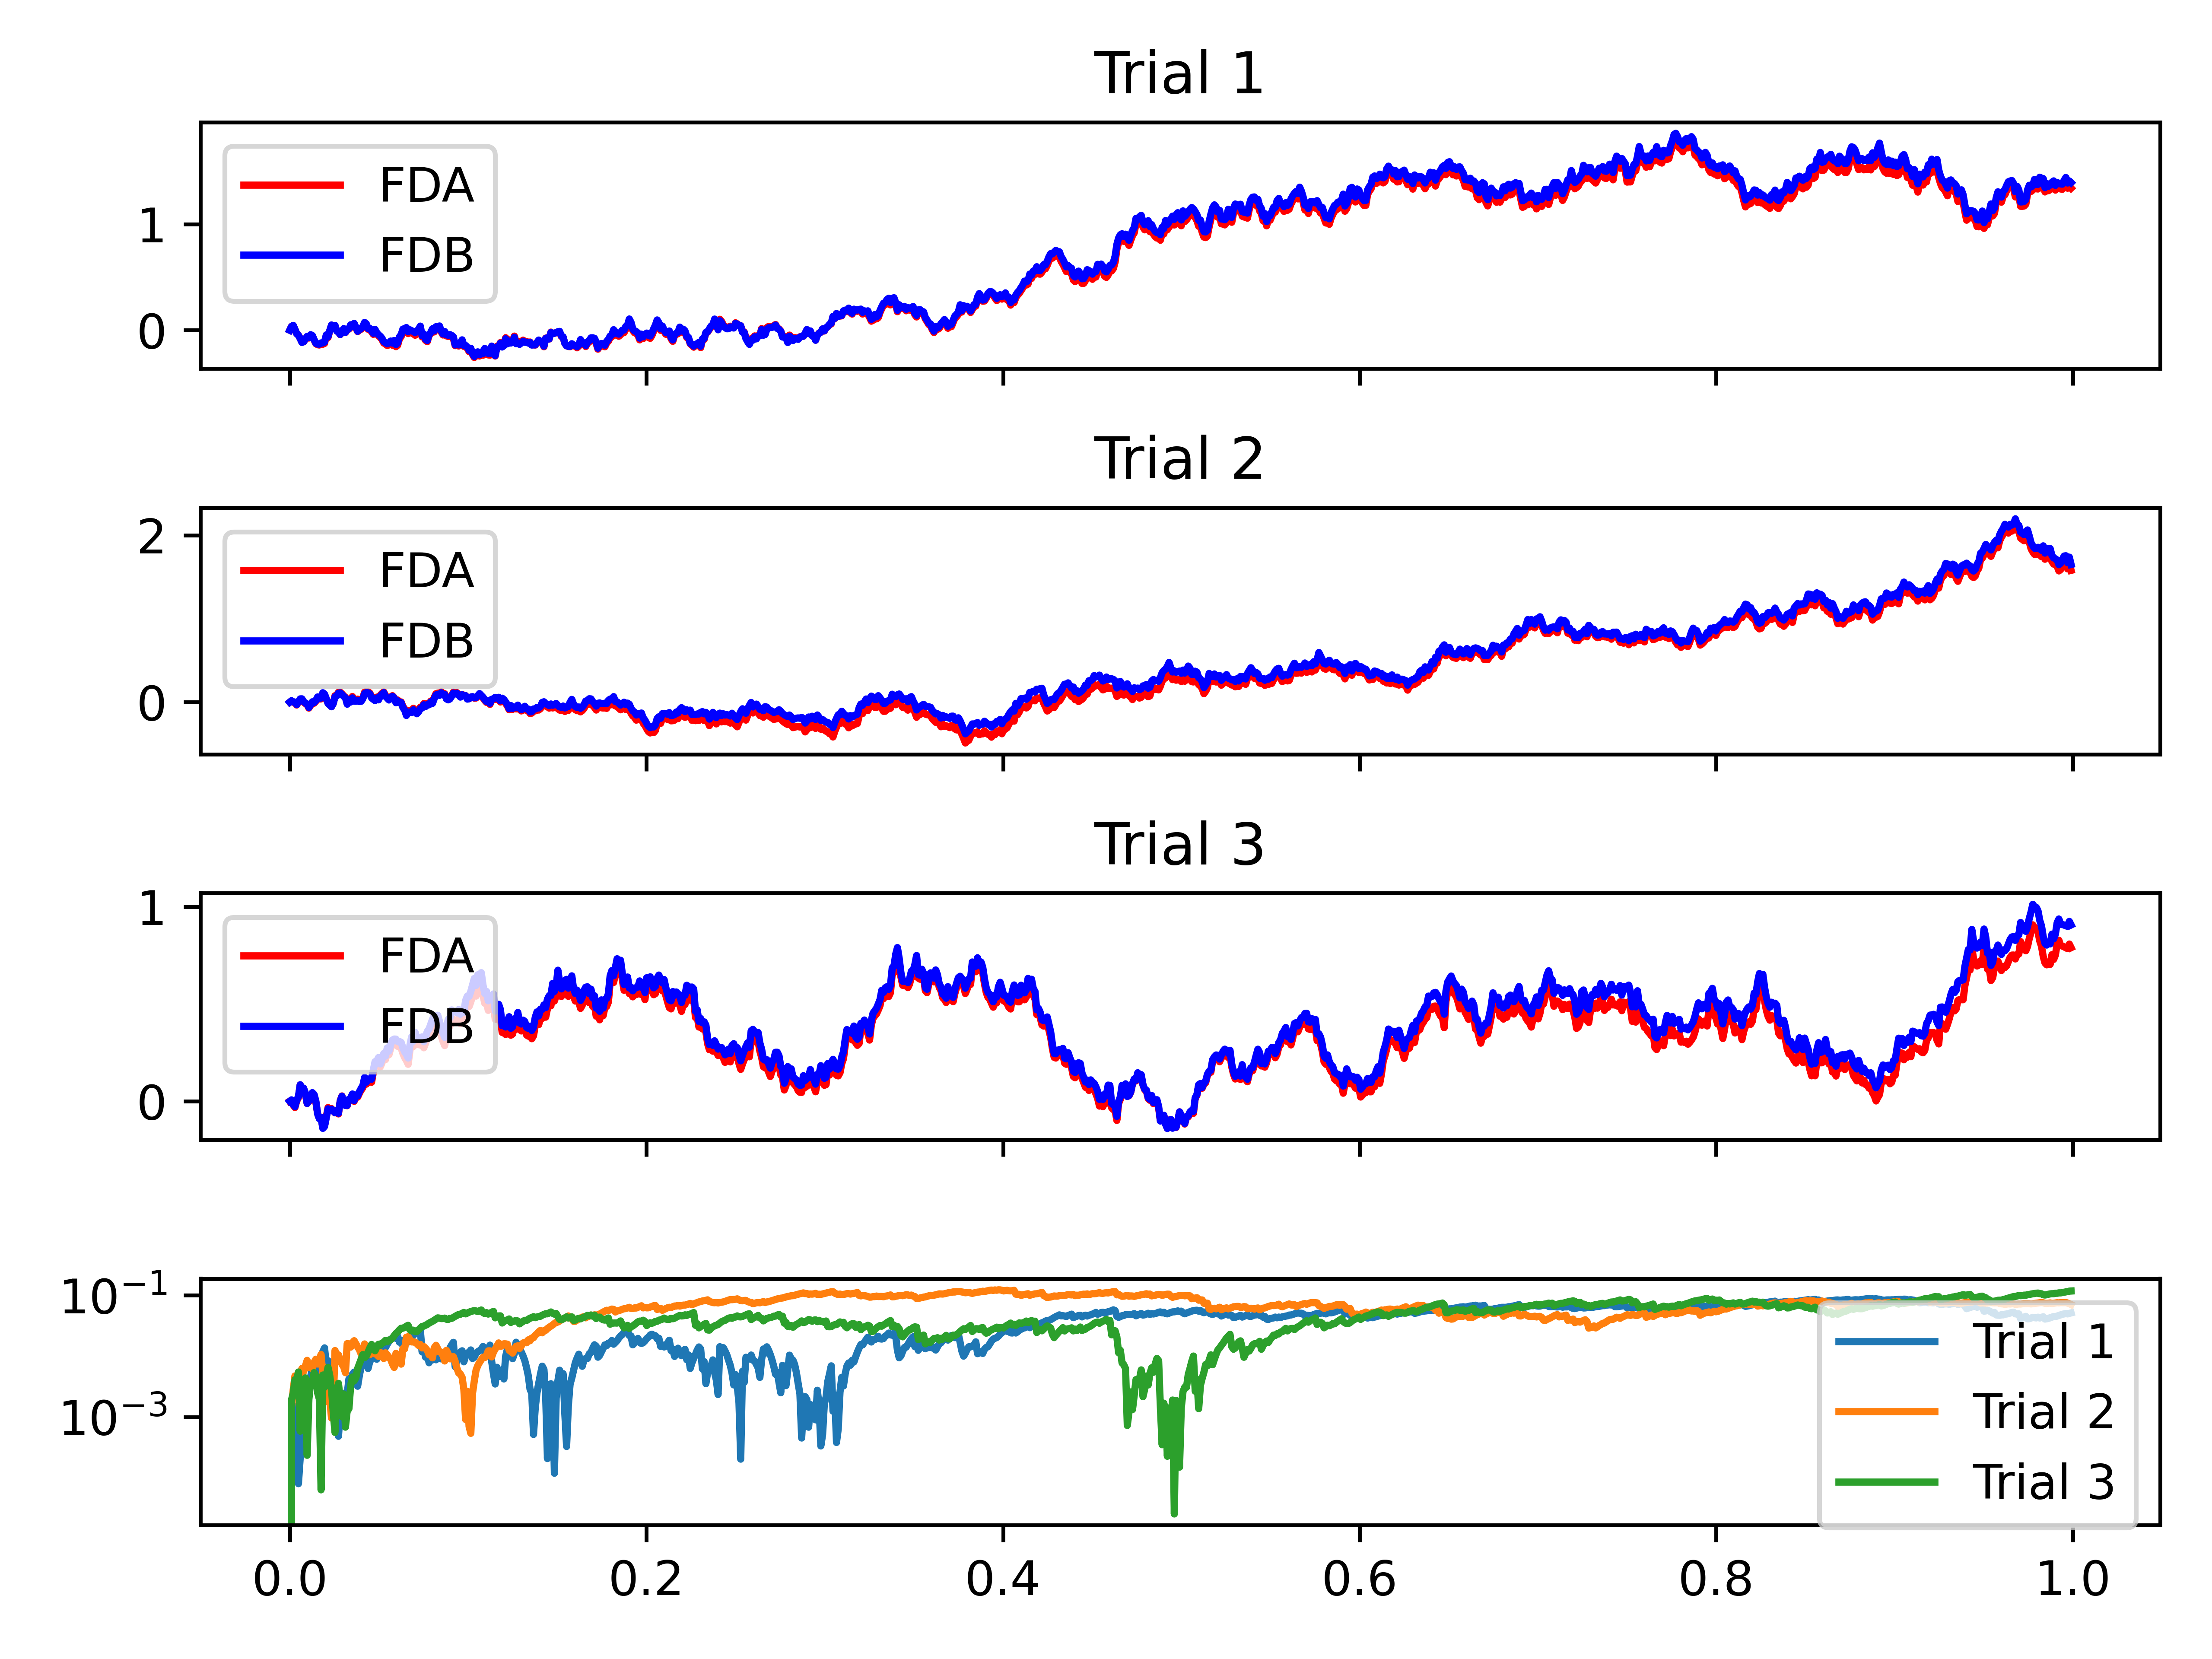
\includegraphics[width=\textwidth]{prob7_pb.png}
    \caption{Numerical Results for problem 7 part b}
    \label{fig:p7pb}
\end{figure}

\begin{figure}[th]
    \centering
    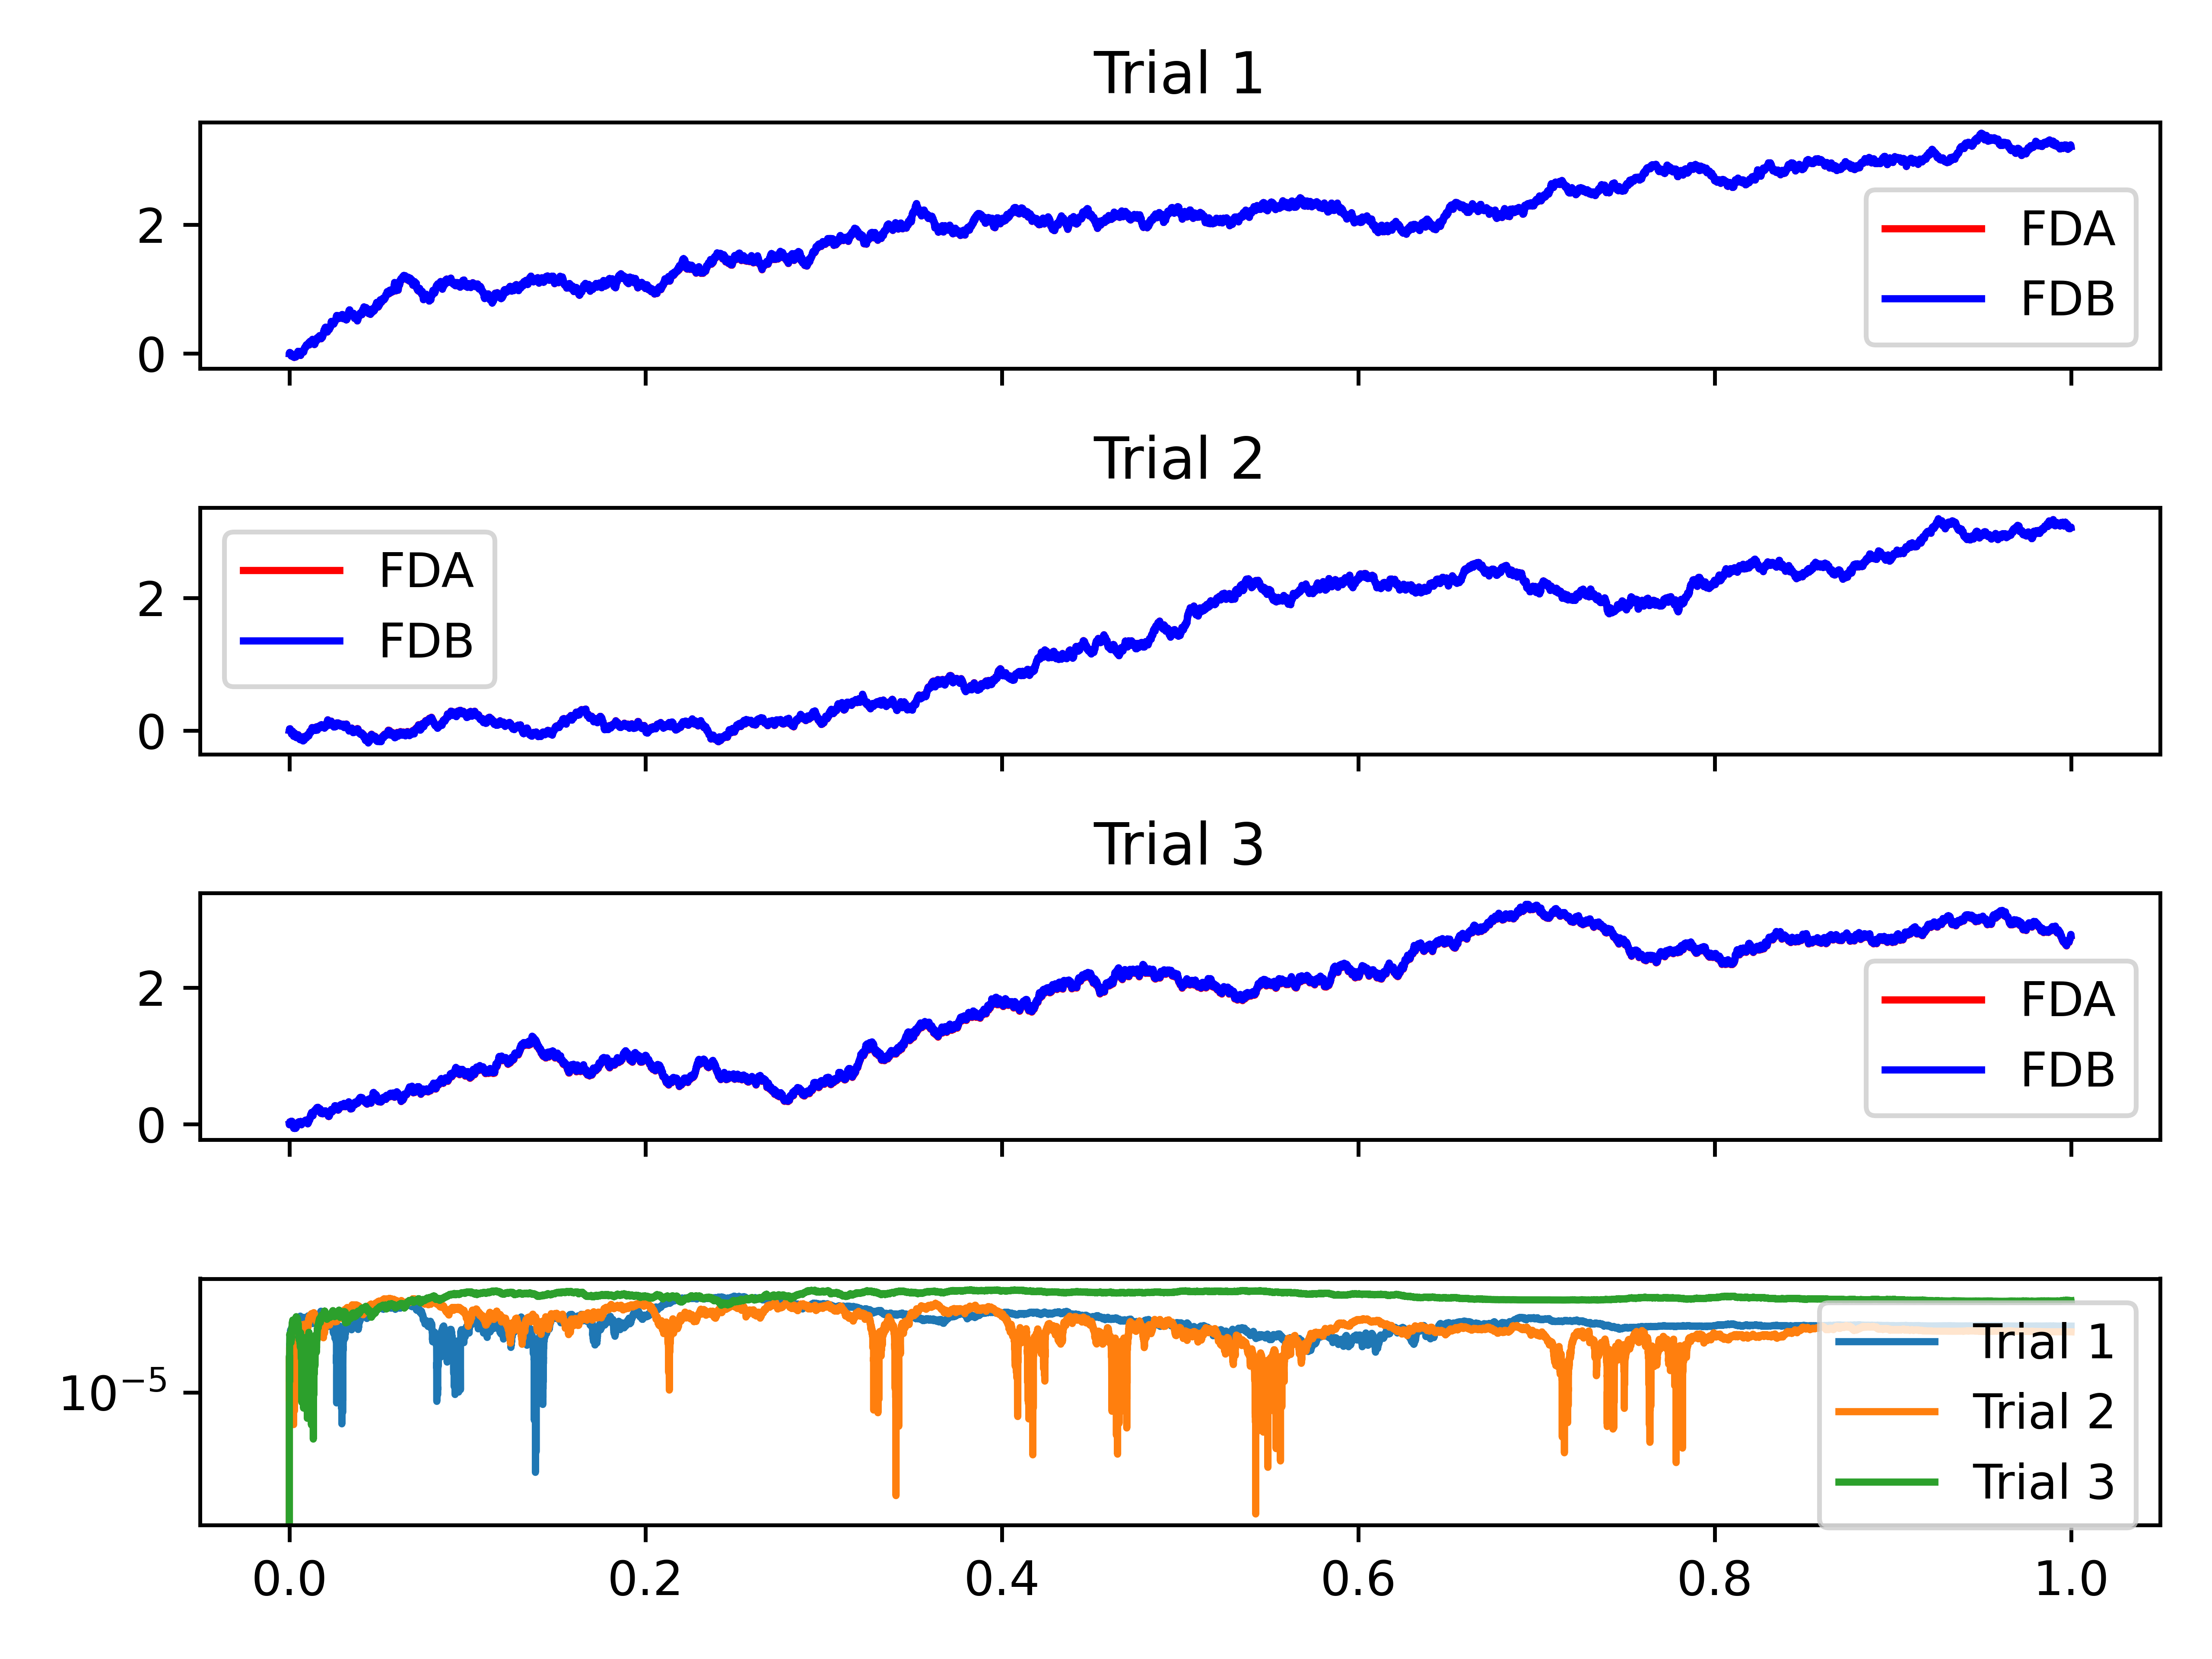
\includegraphics[width=\textwidth]{prob7_pc.png}
    \caption{Numerical Results for problem 7 part c}
    \label{fig:p7pc}
\end{figure}

\section{Refined Sampling for Wiener Process}
See Figure \ref{fig:p8}

\begin{figure}[th]
    \centering
    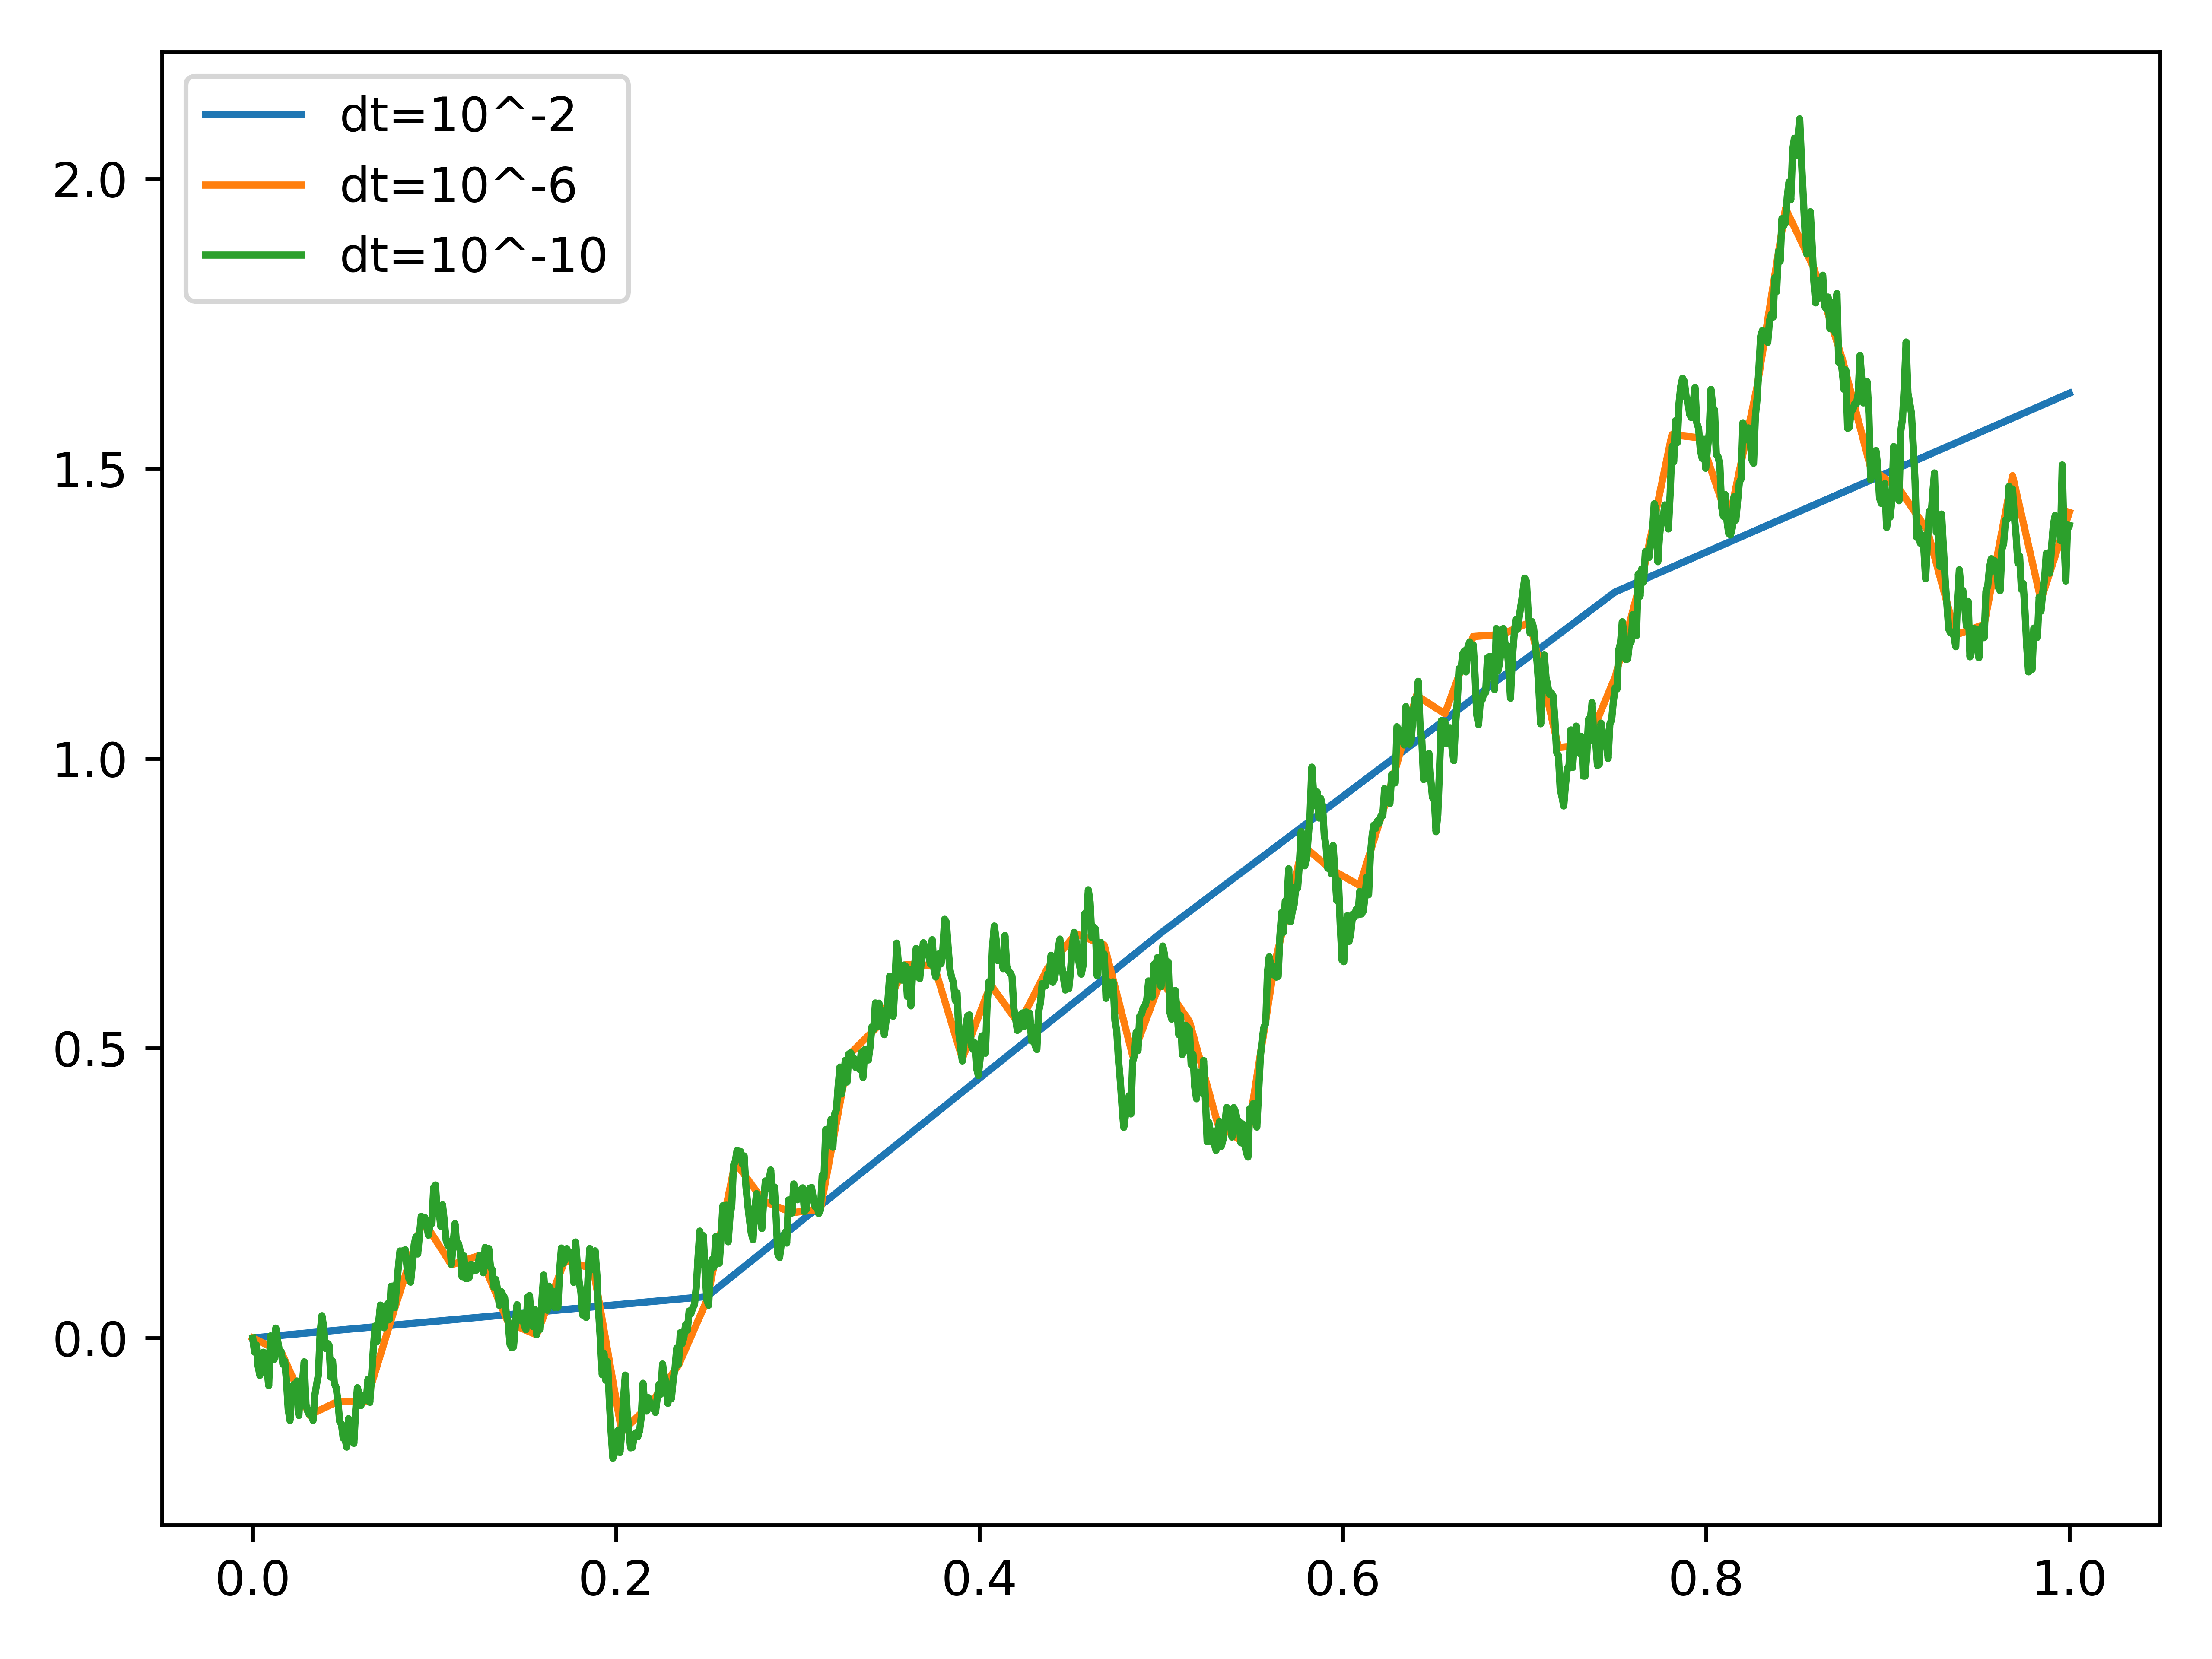
\includegraphics[width=\textwidth]{prob8.png}
    \caption{Numerical Results for problem 8}
    \label{fig:p8}
\end{figure}

\end{document}
